\documentclass[10pt, compress, aspectratio=169]{beamer}

\usetheme[numbering=fraction, progressbar=none, titleformat=smallcaps]{metropolis}
\usepackage{booktabs}
\usepackage{array}
\usepackage{listings}
\usepackage{graphicx}
\usepackage[scale=2]{ccicons}
\usepackage{url}
\usepackage{relsize}
\usepackage{wasysym}

\usepackage{pgfplots}
\usepgfplotslibrary{dateplot}

\lstset{ %
  backgroundcolor={},
  basicstyle=\ttfamily\footnotesize,
  breakatwhitespace=true,
  breaklines=true,
  captionpos=n,
  commentstyle=\color{orange},
  escapeinside={\%*}{*)},
  extendedchars=true,
  frame=n,
  keywordstyle=\color{orange},
  language=C++,
  rulecolor=\color{black},
  showspaces=false,
  showstringspaces=false,
  showtabs=false,
  stepnumber=2,
  stringstyle=\color{gray},
  tabsize=2,
  keywords={thrust,plus,device_vector, copy,transform,begin,end, copyin,
  copyout, acc, \_\_global\_\_, void, int, float, main, threadIdx, blockIdx,
  blockDim, if, else, malloc, NULL, cudaMalloc, cudaMemcpy, cudaSuccess,
  cudaGetLastError, cudaDeviceSynchronize, cudaFree, cudaMemcpyDeviceToHost,
  cudaMemcpyHostToDevice, const, data, independent, kernels, loop,
  fprintf, stderr, cudaGetErrorString, EXIT_FAILURE, for, dim3},
  otherkeywords={::, \#pragma, \#include, <<<,>>>, \&, \*, +, -, /, [, ], >, <}
}

\renewcommand*{\UrlFont}{\ttfamily\smaller\relax}

\graphicspath{{images/}}

\title{Deadlocks, Starvation, Message Passing and others}
\author{\footnotesize Rodrigo Siqueira \\ {\scriptsize siqueira@ime.usp.br}}
\institute{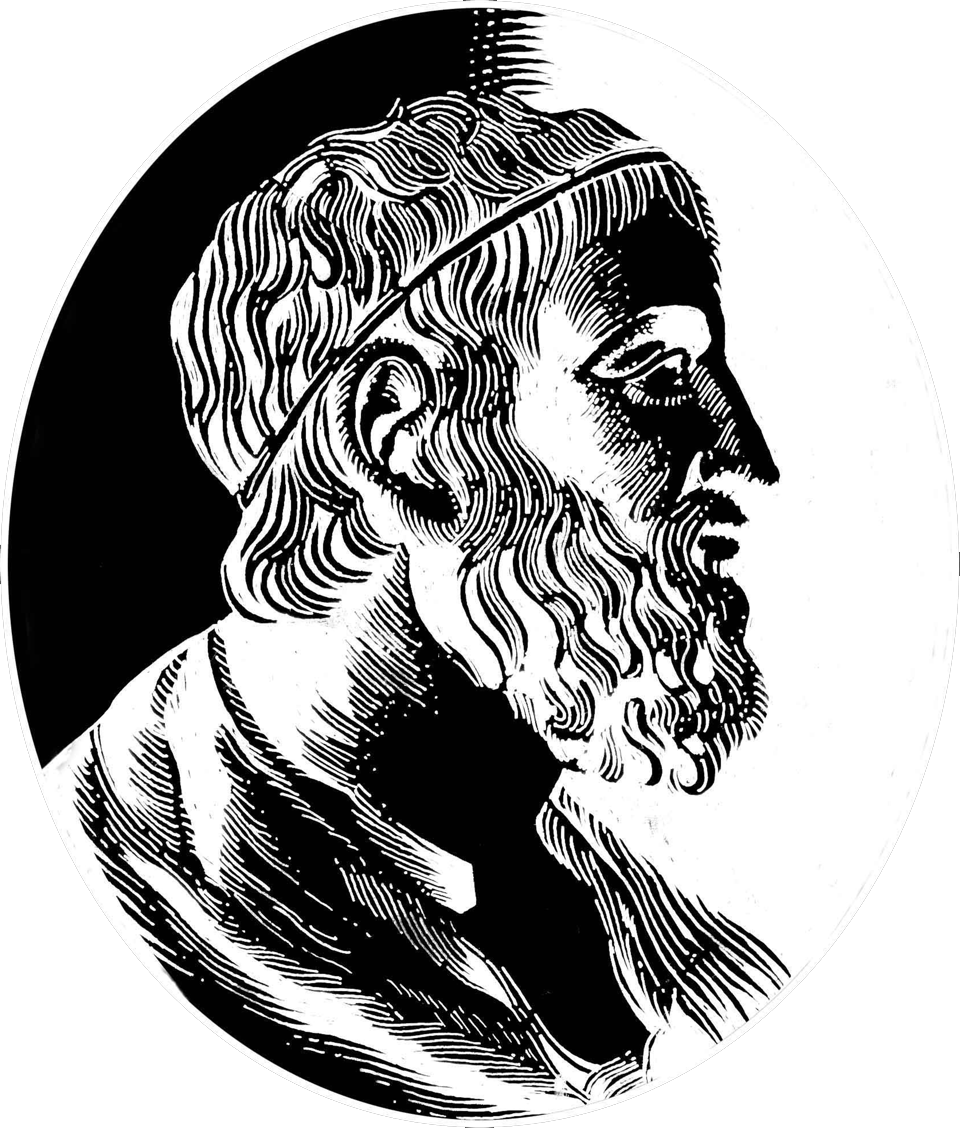
\includegraphics[height=2cm]{imelogo}\\[0.2cm] Department of Computer Science \\ University of São Paulo}

\begin{document}

\maketitle

%------------------------------------------------------------------------------
\section{Introduction}
\begin{frame}{Overview}
  % TODO: Create this section
  \begin{itemize}
    \item Computers...
  \end{itemize}
\end{frame}

%------------------------------------------------------------------------------
\section{Deadlock}
\begin{frame}{What is a deadlock?}
  % TODO: Create an image that shows a situation of deadlock
  \begin{figure}[ht]
    \centering
    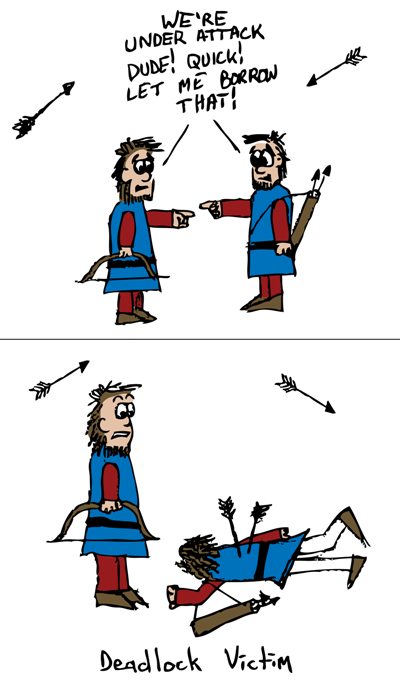
\includegraphics[width=0.3\textwidth, keepaspectratio=true]{images/deadlock.png}
  \end{figure}
\end{frame}

\begin{frame}{Conditions to Deadlock}
  \begin{itemize}
    \item Resource is not preemptable
    \item Resource is not shareable
    \item Process can keep one resource and require another one
    \item Circular wait is possible
  \end{itemize}
\end{frame}

\begin{frame}{Prevent deadlock}
  \begin{itemize}
    \item Should allow the preemption
    \item Avoid multiple exclusion
    \item Avoid keep and wait
    \item Avoid circular wait
  \end{itemize}
\end{frame}

\begin{frame}{Avoid deadlock}
  % TODO: Put some explanations here
\end{frame}

\begin{frame}{Recovery from deadlock}
  \begin{itemize}
    \item Detect
    \item Break
  \end{itemize}
\end{frame}

\begin{frame}{Approaches to handling deadlocks}
  % TODO
\end{frame}

%------------------------------------------------------------------------------
\section{Starvation}
\begin{frame}{What is starvation?}
  % TODO: Make some slides about it
\end{frame}

%------------------------------------------------------------------------------
\section{Message-Passing}

\subsection{PID to address}
\begin{frame}{PID to address}
  \begin{itemize}
    \item Message-to-Message
      \begin{itemize}
        \item Complex
        \item Flexible
      \end{itemize}
    \item Directly to process buffer
      \begin{itemize}
        \item Simple
        \item Inflexible
      \end{itemize}
  \end{itemize}
\end{frame}

\subsection{Message passing with unblocking receive}
\begin{frame}{Message passing with unblocking receive}
  \begin{itemize}
    \item Auxiliary process
    \item Poll on queues
    \item Simultaneously queue read
  \end{itemize}
\end{frame}

\subsection{Message queue blocking in sending}
\begin{frame}{Message queue blocking in sending}
  % TODO: Put some informations here
\end{frame}

\subsection{RPC}
\begin{frame}{RPC}
  % TODO: Put some informations here
\end{frame}

%------------------------------------------------------------------------------
\section{Synchronization}
\begin{frame}{What is synchronization?}
  % TODO: Create some slides to this
\end{frame}

\begin{frame}{Patterns}
  \begin{itemize}
    \item Producer-Consumer
    \item Client-Server
    \item Mutex
  \end{itemize}
\end{frame}

%------------------------------------------------------------------------------
\section{Semaphores}
\begin{frame}{Real life example}
  % TODO: Create a bunch of image to illustrate the situation of a guy that
  % have to wait for the toilet key in the gas station
   \begin{figure}[ht]
    \centering
    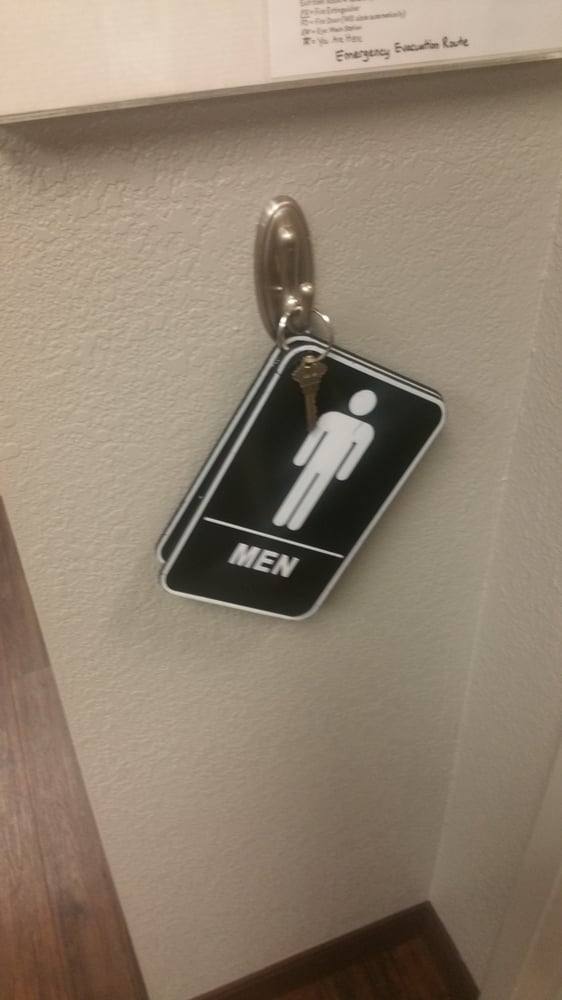
\includegraphics[width=0.3\textwidth, keepaspectratio=true]{images/semaphore.jpg}
  \end{figure}
\end{frame}

\begin{frame}{Operations}
  \begin{itemize}
    \item Create
    \item Wait
    \item Signal
  \end{itemize}
\end{frame}

%------------------------------------------------------------------------------
\section{About this presentation}
\begin{frame}[standout]
  % TODO: Improve it
   \begin{center}\ccbysa\end{center}
\end{frame}


\maketitle

\end{document}
